\scanpage{50}
\mspage{4}
\figure{
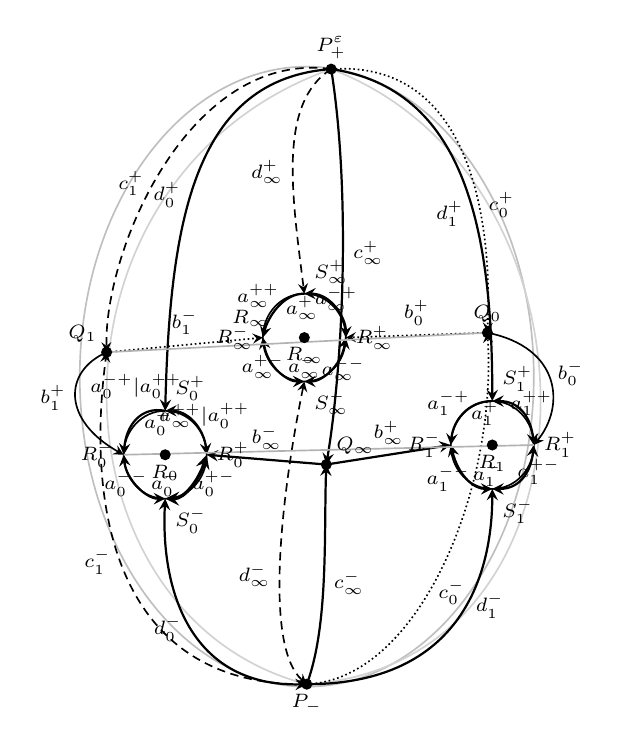
\begin{tikzpicture}[x=.62cm,y=.62cm,>=stealth,every node/.style={font=\scriptsize},line width=.6pt]
\coordinate (Pp) at (5.2,13.2); \coordinate (Pm) at (4.7,.6);
\coordinate (Qz) at (8.4,7.8); \coordinate (Qo) at (.6,7.4); \coordinate (Qi) at (5.1,5.1);
\coordinate (Rz) at (1.8,5.3); \coordinate (Ro) at (8.5,5.5); \coordinate (Ri) at (4.65,7.7);
\draw[gray!50] (4.7,6.9) ellipse (4.65 and 6.35);
\draw[gray!35] (Pp) .. controls (-1,11) and (-.7,2) .. (Pm) .. controls (11,1) and (11,11) .. (Pp);
\draw[densely dashed,->] (Pp) .. controls (2.3,13.6) and (.55,9.5) .. (Qo) node[pos=.55,left] {$c_1^+$};
\draw[densely dashed,->] (Pm) .. controls (.9,.55) and (.15,4) .. (Qo) node[pos=.55,left] {$c_1^-$};
\draw[densely dotted,->] (Pp) .. controls (8.1,13.4) and (8.5,10) .. (Qz) node[pos=.64,right] {$c_0^+$};
\draw[densely dotted,->] (Pm) .. controls (7,.7) and (8.6,4.6) .. (Qz) node[pos=.43,right] {$c_0^-$};
\draw[thick,->] (Pp) .. controls (5.6,10.7) and (5.45,7.2) .. (Qi) node[pos=.45,right] {$c_\infty^+$};
\draw[thick,->] (Pm) .. controls (5.15,1.8) and (5.05,3.7) .. (Qi) node[pos=.48,right] {$c_\infty^-$};
\draw[thick,->] (Pp) .. controls (2.4,13.0) and (1.9,10.1) .. (1.8,6.2) node[pos=.56,left] {$d_0^+$};
\draw[thick,->] (Pp) .. controls (7.9,12.8) and (8.5,10) .. (8.5,6.4) node[pos=.6,left] {$d_1^+$};
\draw[densely dashed,->] (Pp) .. controls (4.1,12.5) and (4.4,10.6) .. (4.65,8.6) node[pos=.56,left] {$d_\infty^+$};
\draw[thick,<->] (Pm) .. controls (2.4,.55) and (1.7,2.4) .. (1.8,4.4) node[pos=.5,left] {$d_0^-$};
\draw[thick,->] (Pm) .. controls (7.9,.6) and (8.5,2.9) .. (8.5,4.6) node[pos=.55,right] {$d_1^-$};
\draw[densely dashed,<->] (4.65,6.8) .. controls (4.2,4.6) and (3.8,1.4) .. (Pm) node[pos=.55,left] {$d_\infty^-$};
\draw[->,densely dotted] (Qo)--(3.8,7.7) node[midway,above] {$b_1^-$};
\draw[->,densely dotted] (Qz)--(5.5,7.7) node[midway,above] {$b_0^+$};
\draw[thick,->] (Qi)--(2.65,5.3) node[midway,above] {$b_\infty^-$};
\draw[thick,->] (Qi)--(7.65,5.5) node[midway,above] {$b_\infty^+$};
\draw[->] (Qo) .. controls (-.3,7) and (-.3,6) .. (.95,5.3) node[pos=.5,left] {$b_1^+$};
\draw[->] (Qz) .. controls (9.9,7.5) and (10,6.3) .. (9.35,5.5) node[pos=.45,right] {$b_0^-$};
\draw (Rz) ellipse (.85 and .9); \draw (Ro) ellipse (.85 and .9); \draw (Ri) ellipse (.85 and .9);
\draw[->,thick] (1.8,6.2) .. controls (1.3,6.3) and (1,5.9) .. (.95,5.3);
\draw[<->,thick] (1.8,6.2) .. controls (2.3,6.2) and (2.6,5.8) .. (2.65,5.3);
\draw[<->,thick] (.95,5.3) .. controls (1,4.8) and (1.4,4.4) .. (1.8,4.4);
\draw[<->,very thick] (2.65,5.3) .. controls (2.5,4.8) and (2.2,4.4) .. (1.8,4.4);
\draw[->,thick] (8.5,6.4) .. controls (8,6.4) and (7.7,6) .. (7.65,5.5);
\draw[<->,thick] (8.5,6.4) .. controls (9.1,6.4) and (9.3,6) .. (9.35,5.5);
\draw[<->,thick] (7.65,5.5) .. controls (7.8,4.9) and (8.1,4.6) .. (8.5,4.6);
\draw[<->,thick] (8.5,4.6) .. controls (9.1,4.6) and (9.3,5) .. (9.35,5.5);
\draw[->,thick] (4.65,8.6) .. controls (4.2,8.6) and (3.9,8.1) .. (3.8,7.7);
\draw[<->,thick] (4.65,8.6) .. controls (5.2,8.6) and (5.5,8.1) .. (5.5,7.7);
\draw[<->,thick] (3.8,7.7) .. controls (3.9,7.1) and (4.3,6.8) .. (4.65,6.8);
\draw[<->,thick] (5.5,7.7) .. controls (5.4,7.1) and (5,6.8) .. (4.65,6.8);
\draw[gray!60] (Qo)--(Qz) (.95,5.3)--(9.35,5.5);
\foreach \p in {Pp,Pm,Qz,Qo,Qi,Rz,Ro,Ri} \fill (\p) circle (2pt);
\node[above] at (Pp) {$P_{+}^{\deleted{\unsure{\varepsilon}}}$}; \node[below] at (Pm) {$P_-$};
\node[above left] at (Qo) {$Q_1$}; \node[above] at (Qz) {$Q_0$}; \node[above right] at (Qi) {$Q_\infty$};
\node[below] at (Rz) {$R_0$}; \node[below] at (Ro) {$R_1$}; \node[below] at (Ri) {$R_\infty$};
\node[left] at (.95,5.3) {$R_0^-$}; \node[right] at (2.65,5.3) {$R_0^+$};
\node[left] at (7.65,5.5) {$R_1^-$}; \node[right] at (9.35,5.5) {$R_1^+$};
\node[left] at (3.8,7.7) {$R_\infty^-$}; \node[right] at (5.5,7.7) {$R_\infty^+$};
\node[above right] at (1.8,6.2) {$S_0^+$}; \node[below right] at (1.8,4.4) {$S_0^-$};
\node[above right] at (8.5,6.4) {$S_1^+$}; \node[below right] at (8.5,4.6) {$S_1^-$};
\node[above right] at (4.65,8.6) {$S_\infty^+$}; \node[below right] at (4.65,6.8) {$S_\infty^-$};
\node at (1.2,6.7) {$\unsure{a_0^{-+}|a_0^{++}}$}; \node at (2.6,6.1) {$\unsure{a_\infty^{++}|a_0^{++}}$};
\node at (2.8,4.7) {$\unsure{a_0^{+-}}$}; \node at (1,4.7) {$\unsure{a_0^{--}}$};
\node at (1.65,5.95) {$a_0^+$}; \node at (1.8,4.7) {$a_0^-$};
\node at (7.6,6.35) {$\unsure{a_1^{-+}}$}; \node at (9.3,6.35) {$a_1^{++}$};
\node at (9.45,4.95) {$\unsure{a_1^{+-}}$}; \node at (7.6,4.8) {$a_1^{--}$};
\node at (8.35,6.15) {$a_1^+$}; \node at (8.4,4.9) {$\unsure{a_1^-}$};
\node at (3.7,8.55) {$a_\infty^{++}$}; \node at (5.3,8.5) {$\unsure{a_\infty^{-+}}$};
\node at (5.45,7.05) {$a_\infty^{--}$}; \node at (3.8,7.1) {$\unsure{a_\infty^{+-}}$};
\node at (4.6,8.3) {$a_\infty^+$}; \node at (4.65,7.1) {$a_\infty^-$};
\node at (3.55,8.1) {$\deleted{\unsure{R_\infty}}$};
\end{tikzpicture}
}
On introduit
\[
(16)\quad\left\{\begin{array}{l}
Q_i\ (i\in\unsure{J|I})\text{ antipodique de }R_i\ \inserted{(=-R_i)}\\
R_i^\omega\in U_i\quad(i\in\unsure{J|I},\omega\in\uline{\omega})\\
P_\varepsilon\ \deleted{\unsure{\in}}\quad(\varepsilon\in\uline{\varepsilon}=\unsure{\pi_0|\Pi_0}(\Sigma\setminus\Sigma_{\mathbb R}))\\
S_i^\varepsilon
\end{array}\right.
\]
où $P_\varepsilon$ est défini par
\[
(17)\qquad\{P_\varepsilon\}=\Delta\cap(\Sigma-\Sigma_{\mathbb R})_\varepsilon
\]
\deleted{\unsure{des} $R_i^\omega\in U_{i\mathbb R}\unsure{\simeq\omega}$}
et $\unsure{R_{i\omega}|R_i^\omega}$ est défini ainsi

On a une bijection canonique
\[
(18)\qquad U_{i\mathbb R}\overset{\mathrm{def}}=\underbrace{U_i\cap\overline T_{\Sigma_{\mathbb R},R_i}}_{T^U_{\Sigma_{\mathbb R},R_i}}\simeq\omega
\]
\unsure{sur} \deleted{\unsure{cette}} variété \inserted{$\Sigma_{\mathbb R}$} de dim 1, l'une des orientations de celle-ci en les points $R_i$ (donc globalement) est en corr. biunivoque avec l'une des deux directions orientées tangentes.
\margin{
\[
(19)\quad S_i^\varepsilon\in U_i\cap\overline T\Sigma_i=T^U\Sigma_i\ \deleted{\unsure{de}}
\]
où $\Sigma_i$ est le grand cercle déterminé par les $P_\varepsilon$ et $Q_i$; on a $T^U\Sigma_i\simeq\uline{\varepsilon}$. Car les deux directions tangentes à $\Sigma_i$ en $R_i$ se distinguent suivant les deux hémisphères $\varepsilon\in\uline{\varepsilon}=\unsure{\pi_0|\Pi_0}(\Sigma\setminus\Sigma_{\mathbb R})$.
}
\margin{\uline{NB} Il faudrait introduire $\widetilde\Sigma^\varepsilon$ $(\varepsilon\in\uline{\varepsilon})$, les deux hémisphères sur $\widetilde\Sigma$, le choix des $S_i^\varepsilon$ est caractérisé par $S_i^\varepsilon\in\widetilde\Sigma^\varepsilon$.}
On a fait la figure en indexant
\[
\unsure{J|I}=\{0,1,\infty\}\qquad \uline{\omega}=\{+1,-1\}
\]
et en choisissant une orientation sur \unsure{le}, i.e.
\[
\uline{\omega}\simeq\{+1,-1\},\quad\text{d'où }\varepsilon\simeq\{+1,-1\}.
\]
\margin{$+$ donné par la perm. circulaire $1\to2\to3$\quad $-$ par l'inverse.}
\deleted{On définit des \unsure{arcs de cercle} sur $\widetilde\Sigma$}
\deleted{\inserted{choisit des chemins}}
\deleted{liant des points de $\widetilde\Sigma$}
\deleted{$(19)\qquad a_i^\omega,\ b_i,\ c_i^\omega$}
\deleted{On choisit dorénavant une orientation de $\unsure{\Sigma}$ (points intérieurs des \unsure{géodésiques}) (pour les $b_i^\omega$)}
\deleted{\unsure{notations pléthoriques}, \illegible{1}}
\margin{49}
